%%%%%%%%%%%%%%%%%%%%%%%%%%%%%%%%%%%%%%%%%%%%%%%%%%%%%%%%%%%%%%%%%%%%%%%%%%%%%%%%
% Template for USENIX papers.
%
%%%%%%%%%%%%%%%%%%%%%%%%%%%%%%%%%%%%%%%%%%%%%%%%%%%%%%%%%%%%%%%%%%%%%%%%%%%%%%%%

\documentclass[letterpaper,twocolumn,10pt]{article}
\usepackage{usenix-2020-09}

% to be able to draw some self-contained figs
\usepackage{tikz}
\usepackage{amsmath}
\usepackage{hyperref}
\usepackage[normalem]{ulem}
\usepackage{listings, listings-rust}
\usepackage{xspace}

% BibLaTeX for bibliography
\usepackage[
  backend=biber,
  style=numeric-comp,
  minalphanames=3,
  isbn=false,
  sortcites=true,
  sorting=anyt,
  abbreviate=false,
  url=false,
  doi=false,
  maxnames=99,
  minbibnames=3,
  maxbibnames=99]{biblatex}
\addbibresource{paper.bib}

\newcommand{\sys}{DeCor}
\newcommand{\plinked}{$p_\text{linked}$}
\newcommand{\premnant}{$p_\text{remnant}$}
\newcommand{\uidkey}{$uid_\text{key}$}
\newcommand{\gidkey}{$gid_\text{key}$}
\newcommand\ms[1]{\textcolor{red!55!blue}{[malte: {#1}]}}
\newcommand\lyt[1]{\textcolor{green!55!blue}{[lyt: {#1}]}}
\newcommand{\tabitem}{~~\llap{\textbullet}~~}
%\renewcommand\lyt[1]{}
\newcommand{\eg}{{e.g.},\xspace}
\newcommand{\ie}{{i.e.},\xspace}


\definecolor{codegreen}{rgb}{0,0.4,0}
\definecolor{codegray}{rgb}{0.5,0.5,0.5}
\definecolor{codepurple}{rgb}{0.58,0,0.82}
\definecolor{backcolour}{rgb}{0.95,0.95,0.92}

\lstdefinestyle{rust}{
    %backgroundcolor=\color{backcolour},
    commentstyle=\color{codegreen},
    keywordstyle=\color{magenta},
    numberstyle=\tiny\color{codegray},
    stringstyle=\color{codepurple},
    basicstyle=\ttfamily\scriptsize,
    breakatwhitespace=false,
    breaklines=true,
    captionpos=b,
    keepspaces=true,
    numbers=left,
    numbersep=3pt,
    showspaces=false,
    showstringspaces=false,
    showtabs=false,
    tabsize=2
}
\lstset{style=rust}

%-------------------------------------------------------------------------------
\begin{document}
%-------------------------------------------------------------------------------

%don't want date printed
\date{}

% make title bold and 14 pt font (Latex default is non-bold, 16 pt)
\title{\Large \bf \sys{}: Ensuring the Right To Be Forgotten in Web Applications}

%for single author (just remove % characters)
%\author{
%{\rm Lillian Tsai}\\
%MIT
%\and
%{\rm Malte Schwarzkopf}\\
%Brown University
%% copy the following lines to add more authors
%\and
%{\rm Eddie Kohler}\\
%Harvard University
%} % end author

\author{
{\rm Anonymous Authors}\\
} % end author

\maketitle

\begin{abstract}
    Web applications face increasing legal and user demands to properly protect and manage user
    data, whether through supporting user's right to be forgotten, removing unnecessary or old user
    data, or moderating user content.
    %
    Meeting these demands to \emph{mask} data requires that applications perform the appropriate
    data transformations to sufficiently de-identify or modify data, while still retaining the data
    required for application utility or legal purposes. Because such transformations are necessarily
    application-specific and require handling complex data correlations, today's applications often
    forgo these transformations, or use ad-hoc methods with unclear guarantees to achieve them.
    %

    To help developers flexibly support data masking transformations in new and existing
    applications, we design and implement \sys, a system that takes as input a high-level
    specification of a transformation, and automatically applies it to the application database.
    \sys relies on the key abstractions of application \emph{entity graphs} and \emph{ghost
    entities}, which allow developers to express and automate practical transformations without
    onerous labor.
\end{abstract}

\iffalse
%
\name is a new data ownership paradigm for web services in which users subscribe to
services by granting a \emph{lease} of their data, instead of having a permanent account.
%
When the lease ends, the user switches from an identity-revealing
subscribed mode into a privacy-preserving unsubscribed mode, where the
service only retains anonymized data about them.
%
This paradigm strikes a balance between current practices that give services control over user
    data with low user privacy; and the opposite extreme that decouples user data from
    services for strong privacy, but breaks current business models and reduces service utility.
%achieves better user privacy and data protection than today's services, 
%but without making impractical assumptions or breaking current business models.
%
Under \name, users withdraw from a service without permanently losing access,
as they can resubscribe at any time, and one user's withdrawal does not affect
the service's utility for others.

%
A prototype design and implementation for \name suggests it can be realized
efficiently and with low burden for application developers.
%
%\ms{We should give our paradigm a name!}

%The paper proposes a new web application \emph{subscription paradigm},  Users flexibly switch between a privacy-preserving unsubscribed mode and an
%identity-revealing subscribed mode at any time without permanently losing their data. 
%This subscription paradigm strikes a balance between applications having complete ownership of user
%data, and completely decoupling user data from applications at the cost of application utility. 
%To solve the complex data retention and de-identification challenges associated with subscription,
%we design \name{}, a practical system that provides abstractions and mechanisms to help
%developers of databased-backed web applications achieve correct, privacy-compliant user
%unsubscription and resubscription without onerous labor.
\fi

%-------------------------------------------------------------------------------
\section{Introduction}
%-------------------------------------------------------------------------------

Web application users are more aware of their data privacy rights than ever before. 
Laws such as the European Union's General Data Protection Regulation (GDPR)~\cite{eu:gdpr} and
California's Consumer Privacy Act (CCPA)~\cite{ca:privacy-act} codify users' rights to 
data ownership, granting users the right to request erasure of information related to them.
%
Public news around web services increasingly emphasize the dangers of leaving private data on the
web: embarrassing or compromising details from the past has reemerged, web applications have 
suffered data leaks or hacks, and private data has be shared by web applications without the user's
knowledge or explicit consent~\cite{nytimes:fb, npr:data}.

%
For the first time, companies face both legal and societal demand to support \emph{unsubscription}
of users from their services. Users have the right to unsubscribe at any time, preventing 
idle or unused accounts from retaining personal data indefinitely, and regaining control over who
can access their data. 
%

%
Unsubscription, however, is only half the story. Users cannot truly regain their data rights if they
are impeded from exercising them.  In order to claim that users have regained ownership of their
data, users must be freely able to exercise their right to be forgotten. In particular, they should
not have to pay a high price in order in order to unsubscribe whenever they wish: web services
should not raise barriers to unsubscription that prevent users from choosing to do so, when they
would have otherwise. These barriers can take several forms, from UI choices that hide paths to
unsubscription, to the threat of permanent deletion of years or even decades of accumulated
application data.

To empower users to freely exercise their data rights, web applications must allow users to easily
unsubscribe \emph{and resubscribe} as they wish, switching between a privacy-preserving unsubscribed
mode and an identity-revealing subscribed mode at any time without permanently losing their data, or
needing to maintain their account data themselves. 
%
With this model of flexible privacy, the balance of data ownership flips. Applications no longer
control users' data choices by demanding that users choose between indefinitely giving up their data
to use the application, or permanently losing their data and application utility.
Instead, users lease out their data for limited periods of time in exchange for the ability to use the application for 
that period, and lose no application utility between leases.
%\lyt{Users could do this without
%application support by themselves by programmatically setting a personal reminder to ``unsubscribe
%after x days'' every time they create an account.}
%

In the rest of this paper, we describe the current unsubscription and resubscription support (and
lack of support) in today's web applications, and the challenges of doing so correctly.
We then describe \sys, a system that provides abstractions and mechanisms
that help developers of databased-backed web applications achieve correct,
privacy-compliant user unsubscription and resubscription without onerous labor, and without adding
undue overheads.

%-------------------------------------------------------------------------------
\section{Related Work}
%-------------------------------------------------------------------------------
\label{sec:related}

%
Protecting personal data in web services is a long-standing research direction.
%
\textbf{Decentralized platforms} such as Solid~\cite{solid}, BSTORE~\cite{bstore},
Databox~\cite{databox} and others~\cite{diy, amber, oort, w5, blockstack}
seek to put data directly under user control.
%
These systems give users power to control access, and often delete or modify, their
own data, but they burden users with maintaining infrastructure, typically lack the
capacity for useful application features based on server-side compute, and they break
the current, ad-based application revenue model.
%
In contrast, data disguising helps application developers support privacy
transformations without changing the application data model or business model,
and allows today's server-side processing.
%

%
Other platforms attest that server-side processing respects
\textbf{user-defined policies} over their data, via cryptographic means~\cite{zeph}
or systems security mechanisms~\cite{riverbed}.
%
The application functionality is typically restricted, in terms of the feasible
operations (\eg additively homomorphic ones) and in whether data with different policies
can be combined.
%
Data disguising only provides assurances about data privacy after the application has
disguised the data, but in exchange allows unrestricted application functionality
without any overhead.
%

%
Other systems enforce developer-specified \textbf{visibility and access control policies}
based on information flow control (IFC)~\cite{static, jeeves, jif, hails, ifdb},
authorized views~\cite{oracle} or per-user views~\cite{multiverse}, and rewriting database
queries~\cite{qapla, sieve}.
%
Data disguising transforms the actual data stored, and, unlike these systems, protects
against full server compromise.
%


%
New privacy laws have led researchers to propose \textbf{database designs
for privacy compliance}.
%
These databases track the owner of data objects and erase them on user request, compliant
with \eg the GDPR.
%
They either modify the data layout~\cite{usershards} or use fine-grained information flow
tracking (IFC) to determine PII propagation and restrict access~\cite{schengendb}.
%
Data disguising can be employed for GDPR compliance, but supports broader privacy
transformations that go beyond deleting PII, and requires no ownership tracking or
fine-grained IFC.
%

%
\textbf{Systems for data deletion}, on the other hand, specifically focus on the
challenge of correctly removing a user's to provide them with post-deletion
privacy.
%
While cryptographically-guaranteed deletion is difficult and expensive~\cite{vanish},
practical systems that help developers get deletion right exist.
%
DELF~\cite{delf}, a framework for data deletion at Facebook helps developers write
correct data deletion code, and uses annotations on application edge and object types
to specify a deletion policy.
%
DELF focuses only on data deletion, while data disguising targets broader privacy
transformations, including decorrelation and anonymization.
%
Sypse~\cite{sypse} pseudonymizes user data and partitions personally identifying
information (PII) from other data.
%
Like data disguising, Sypse's design is application-oblivious, and leaves
the specification of what counts as PII to the application.
%
Instead of constantly maintaining data partitions (as Sypse does), data disguising
adapts the application database on disguising and stores encrypted data to
potentially later reveal it.
%

%
Our work shares some ideas with \textbf{encrypted storage systems}.
%
However, the deployment scenarios for these systems assume that all data is
encrypted, which imposes overheads on normal operation and requires application
functionality to live on the client.
%
Support for arbitrary and fully-oblivious operation over encrypted data would
be ideal, but while there is encouraging recent progress on search over encrypted
data and oblivious key-value stores~\cite{dory, snoopy}, the cost is too high for
practical web services.
%
However, data disguising has a similar threat model to CryptDB~\cite{cryptdb},
Mylar~\cite{mylar}, or Keybase~\cite{keybase}, and protects confidentiality of
data under disguise against similar server compromises.
%
Data disguising encrypts only users' data currently under disguise, but is
efficient and still protects inactive users' privacy.
%

%
%Finally, privacy-enhancing techniques like $k$-anonymity, $l$-diversity, and
%differential privacy~\cite{dataminingmodels, differential} can complement
%data disguising.
%%
%Disguises might add differential privacy noise to
%data left in the application DB, for example.
%


%---------------------------

\iffalse
Key ideas:
    pseudonymization
    data partitioning
    synthetic data

Similarities:
- privacy guarantees weaker than DP, no constraints on queries
- pseudonymization --> overwrite a portion or all of data for individual, difficult to reassociate
    only a small fraction of data?
    breaking up objects grouped by user identifier key
    breaking connections between tables (just like )

- try to ensure that database still useful even w/pseudonymization
    synthetic data (ghosts in \name)
- use of in-memory caches to avoid expensive joins (materialized views)

Differences
- design for \name puts data in hands of user, Sypse has a separate partitioned table (not
necessarily )
- Sypse has synthetic data generation instead of ghosts to replace data taken out
    - foreign keys point to random records
    - VS ghost records
    - not developer-specified? might lead to incorrect behavior?
- what are partitions?
    - limited access, the queries will be run against pseudonymized or synthetic data only
    - Detail Database: anything that isn't PII (pseudonymous)
        - perform analysis, data mining, etc. on these
    - PII Database: anything tied to specific individual (username, user identifiers)
        - replaces with surrogate keys
        - geological / biometric information
        - breaking up objects grouped by user identifier key (direct edge policies)
        - breaking connections between tables (non-direct edge policies)
    - backed up separately, different access control mechanisms
- assumes annotated schema, but doesn't actually describe it!!! just says requires analysis, or is
relatively straightforward
    -made automatically through a continuous analysis of the database schema and the data within it,
    visible to users
    - lack of schema discipline in practice (Database decay and how to avoid it.)
    - no understanding of multiple entities and how they relate to each other
- no support for resubscription

Partition strategies:
- split table into multiple tables, additional joins to reconnect different partitions, doubled updates, forgetting requires multiple
updates
- encrypt certain attributes, add as new attributes, encrypted keys stored in user->key mapping: joins limited
- us: we don't care about size of "PII" table --> this data is given to user

Other related work to cite:
- secure/encrypted databases(?)
- differential privacy
- Kraska SchengenDB: A Data Protection Database Proposal.
    - identify all personal data via tracking / relation graphs
    - tables and columns with PII declared w/schema notations
    - purposes restrict what PII you can access
    - sandboxing
    - also has object relation graph
    - we assume that data isn't copied, whereas they support data copies by tracking ownership
    beyond foreign key relationships
- GDPR by compliance: user shard model
- ScrambleDB: ScrambleDB: Oblivious (Chameleon) Pseudonymization-as-a-Service
- Sieve: A Middleware Approach to Scalable Access Control for DatabaseManagement Systems.

\subsection{Decoupling User Data from Web Applications}
Our proposed subscription paradigm contrasts with a model of strong privacy in web applications, in
which the user has complete data ownership (see Figure~\ref{fig:world}b). In proposals for this
model~\cite{solid, amber, w5, blockstack, bstore}, applications must compute on per-user, filesystem-esque
storage, \eg as JavaScript in users' browsers in Solid~\cite{solid}, Blockstack~\cite{blockstack} and
BStore~\cite{bstore}. Applications face the loss of the flexibility and ease of programming over SQL
databases with application-specific schemas, and users must decide on appropriate access control and
authentication policies. As a result, service-side computation and data sharing between users---a
large reason users use applications to begin with---becomes inefficient and impractical.
%
Furthermore, users are burdened with long-term data maintenance and storage: solutions that use PIKE
(\eg Blockstack~\cite{blockstack}) require users to maintain a
master private key, a cumbersome and fragile solution in which losing the key results in permanent
loss of all the user's data.
%
Finally, users must change the way they pay for services, as the current revenue model for
applications relies on access to user data.
\lyt{this might not be a bad thing, though}.

Under the subscription paradigm, applications do not need to access any data outside its own
servers, simplifying the secure storage of this data when users enter privacy-preserving mode.
Applications can operate as they do today, with the current web architecture's performance and
programming flexibility benefits. However, unlike today's model of data privacy in web applications,
users can freely reclaim their their data and privacy whenever they wish.

\subsection{Data Anonymization}

Prior research on k-anonymization, pseudonymization (more for static analysis purposes than used in
web applications).
%\url{https://amnesia.openaire.eu/index.html}
%\url{https://www.aclweb.org/anthology/2020.coling-main.32.pdf}

While psuedo/anonymization
techniques still allow for reidentification/reconstruction attacks), \name provides better
anonymization than prior approaches, which decorrelate only coarsely by associating remnants of data
with a global placeholder for all deleted users, or do not decorrelate at all (e.g., replacing
usernames with a pseudonym, as in the AOL dataset case~\lyt{TODO}%\cite{aol}).

\subsection{Differentially Private Queries}

PINQ, a data analysis platform created by McSherry~\cite{pinq}, provides formal differential privacy
guarantees for any query allowed by the platform.  Data analysts using PINQ can perform
transformations (Where, Union, GroupBy, and restricted Join operations) on the underlying data
records prior to extracting information via aggregations (e.g., counts, sums, etc.) The aggregation
results include added noise to meet the given privacy budget $\epsilon$, ensuring that analysts only
ever receive $\epsilon$-differentially-private results.  PINQ calculates the privacy loss of any
given query based on transformations and aggregations to be performed; if a particular query exceeds
a predefined privacy budget, PINQ refuses to execute the query.

Differential privacy provides a formal framework that defines the privacy loss a user incurs
when the user's data is included in the dataset. However, the setting of differential privacy
that of \name in several important ways.

First, web applications' utility often derives from visibility into individual data records. PINQ
restricts JOIN transformation and exposes information only through differentially-private
aggregation mechanisms. While sufficient for many data analyses, this approach severely hinders web
application functionality. \name supports all application queries, even ones that expose individual
records, such as \texttt{SELECT story.content, story.tag FROM stories LIMIT 10}.
However, this makes formally defining the privacy guarantees of \name more complex than
simply applying DP.  DP provides formal guarantees for results such as sums or averages because such
results are computed using well-defined mathematics, allowing us to neatly capture the total
knowledge gained by the adversary. However, in the world of web applications, the knowledge gained
via queries that may reveal individual data records cannot be so easily defined: adversaries may
learn information from the friends who liked the (ghosted) story, or the time and location the story
was posted.

Thus, we cannot, in general, use the DP approach of asking, ``by how much do answers to adversary
queries change with the presence of a users' decorrelated data?'' While we can precisely define which
data records an adversary sees with and without a user's decorrelated data, we cannot numerically
quantify the knowledge gained by the adversary in the same way as we can quantify the percentage
change to a sum or average.
Instead, \name reduces identifying information in the changes induced by a users' (decorrelated)
data, rather than reducing the amount of change itself.

This is demonstrated by how PINQ and \name differ in disguising entities associated with unique keys.
PINQ restricts JOINs to group by unique keys. As an (imperfect) example, selecting a JOIN of stories
with users via the UID would result in a record, one per UID, which represents the ``group'' of all
stories associated with a user. A normal join would create a separate record per story, each
associated with the user of that UID.

Instead of lumping all matching stories together, \name explodes the users' UID into individual
unique keys (ghosts), one per story. By PINQ's analysis of stable transformations, this leads to
unbounded stability (as the number of different results produced by queries is proportional to the
potentially very large number of stories for that user). In PINQ's DP framework, such unbounded
stability leads to unbounded privacy loss: one users' data could change aggregation results in
``significant'' ways unless huge amounts of noise were added.

\name and PINQ's approaches can be seen as complementary: for queries that are more analytic in nature (for example,
population statistics used by the web application to measure usage or trends), \name can utilize
PINQ's technique to provide differentially private guarantees (for a particular snapshot of the
dataset).  \name's decorrelation, in fact, adds more noise than necessary in these cases: a count
of unique users who posted about cats will be more imprecise because each post by a decorrelated
user is now associated with a unique (ghost) user.

\subsection{Deletion Privacy}
The right to be forgotten has also been formally defined by Garg et
al.~\cite{garg}, where correct deletion corresponds to the notion of
leave-no-trace: the state of the data collection system after a user requests to be forgotten should
be left (nearly) indistinguishable from that where the user never existed to begin with. While
\name uses a similar comparison, Garg et al.'s formalization assumes that users operate
independently, and that the centralized data collector prevents one user's data from influencing
another's.

Potentially other related works:
\begin{itemize}
    \item Deceptive Deletions for protecting withdrawn posts %https://arxiv.org/abs/2005.14113
    %\item "My Friend Wanted to Talk About It and I Didn't": Understanding Perceptions of
        %Deletion Privacy in Social Platforms, user survey https://arxiv.org/pdf/2008.11317.pdf;
        %talk about decoy deletion, prescheduled deletion strategies~\cite{myfw}
    \item Contextual Integrity
    \item ML Unlearning
    \item Database IFC (sensitive data flowing down edges?)
    \item Graph databases
\end{itemize}
\fi

%-------------------------------------------------------------------------------
\section{Design} 
%-------------------------------------------------------------------------------

\subsection{Disguise Specifications.} 
Because disguises are inherently application-specific, the application developer provides disguise
specifications that consist of a set of predicated disguise operations \op{d} to perform during the
disguise.

Operations \op{d} of disguise $d$ take data objects as input and execute updates to application
data.  \sys automatically generates database change records when applying \op{d}. 

Developers describe in the specification which principals an operation's generated database change
record corresponds to.  For example, a database change record generated by removing comment may
correspond to the principal whose ID is referenced by the author column.  

Developers also specify an application-aware pseudoprincipal generation policy, namely how to
generate new user accounts in a manner that the application can handle (e.g., pseudoprincipals may
not have email addresses).

Finally, developers specify which principals are authorized to apply each disguise: enforcing
access control for disguising is left to the application.
\lyt{It seems most reasonable for the application to enforce AC for the disguising API the
application exposes to the client?}

\vspace{6pt}\noindent
Operations come in three forms:
\begin{enumerate}
    \item Modify: change an attribute of the data object.
    \item Remove: delete the data object.
    \item Decorrelate: generate a \emph{pseudoprincipal} $q$, and rewrite the foreign key to original
        principal $p$ from the data object to instead point to $q$.
        A pseudoprincipal may or may not be indistinguishable from a real principal: for example,
        $q$ may not have an associated password.
\end{enumerate}

\noindent For each \op{d}, the application developer specifies:
\begin{itemize}
    \item An associated predicate over the application database that selects \op{d}'s input
        objects in a SQL-like fashion.
    \item The type of operation and its arguments (e.g., which attributes of the data object to
        modify).
    \item The corresponding principal(s) that should have the capability to access \op{d}'s
        generated disguise change or correlation record.
\end{itemize}

%%%%%%%%%%%%%%%%%%%%%%%%%%%%%%%%%%%%%%%%%%%%%%%%%%%%%%%%%%%%%%
\subsection{Database Diffs.}
%%%%%%%%%%%%%%%%%%%%%%%%%%%%%%%%%%%%%%%%%%%%%%%%%%%%%%%%%%%%%%
Every \op{d} produces a \emph{database diff} \tdata{p\delta_i} associated with the disguise instance $\delta$ and a principal $p$. 

Each \tdata{p\delta_i} contains the ID of the disguise instance, the associated principal $p$'s ID,
and a random nonce.
%
In addition to this data, a decorrelation \tdata{p\delta_i} contains the created pseudoprincipal's
ID; a removal \tdata{p\delta_i} contains the removed object's value; and a modification
\tdata{p\delta_i} contains the old and new value of the modified object.

%%%%%%%%%%%%%%%%%%%%%%%%%%%%%%%%%%%%%%%%%%%%%%%%%%%%%%%%%%%%%%
\subsection{Diff Access Control.} 

\head{Securing Access to Database Diffs.} 
\sys secures database diffs with data capabilities \dcapa{p\delta_i}.
\sys represents a data capability \dcapa{p\delta_i} as a symmetric key specific to
the disguise instance and principal.
%
\sys encrypts \tdata{p\delta_i} with the \dcapa{p\delta_i}. The diff's nonce ensures safety against
known-plaintext attacks. 

%%%%%%%%%%%%%%%%%%%%%%%%%%%%%%%%%%%%%%%%%%%%%%%%%%%%%%%%%%%%%%
\head{Securing Disguise History.}
\sys's design may leak information that $\delta_i$ disguised principal $p$ 
because an adversary may learn that ciphertexts for %\dcapa{p\delta_i} and
\tdata{p\delta_i} exist for a particular $p$ and $\delta_i$.
This is a problem: for example, \sys should not store information that a principal $p$ has
invoked GDPR deletion.

To avoid this problem, \sys stores 
%(1) the \dcapa{p\delta_i} ciphertext and (2) 
an array of \tdata{p\delta_i} ciphertexts at random location pointed to by locating capability
\lcapa{p\delta_i}.  This dissociates one disguise applied to a principal $p$ from all other
disguises, so an adversary only ever learns about a single disguise instance if \sys gains
permission to reveal or compose upon that disguise instance.

Note that an adversary without access to any \lcapa{p\delta_i} can learn that $n$ diffs exist for
\emph{some} $p$ and $\delta_i$, but cannot directly identify which $p$ or $\delta_i$.
If an adversary has access to \lcapa{p\delta_i}, the adversary can learn that $\delta_i$
applied to $p$, and the number of \tdata{p\delta_i} diffs for that $p$ and $d$. This metadata is out of scope of our threat model.

%%%%%%%%%%%%%%%%%%%%%%%%%%%%%%%%%%%%%
\head{Storage of \dcapa{p\delta_i} and \lcapa{p\delta_i}.} 
\sys should not store \dcapa{p\delta_i} or \lcapa{p\delta_i}: an adversary could then
learn that $\delta_i$ has applied to principal $p$. Thus, these capabilities must be stored externally,
even when no client speaking for $p$ is currently online.
%
%The only exception to this occurs when $p$ is a pseudoprincipal: in this case, \sys saves a
%(globally accessible) mapping from $p$ to \lcapa{p\delta_i}. This leaks the disguise history of
%pseudoprincipals, but is allowable because pseudoprincipals' data has already been decorrelated from their
%original principal owner.
%
To communicate these capabilities to a client,
\sys emails (or otherwise communicates) \pcapa{p\delta_i} to a party that can authenticate as $p$. 
\lyt{This assumes that every real user must have an email; alternatively, this could be offloaded to
the application.}
%If no email is present (\eg $p$ is a pseudoprincipal), \sys can save a (globally accessible) mapping from $p$ to \lcapa{p\delta_i}; this leaks disguise-principal associations, but
%only for pseudoprincipals whose data is already decorrelated from their original principal owner.

%%%%%%%%%%%%%%%%%%%%%%%%%%%%%%%%%%%%%%%%%%%%%%%%%%%%%%%%%%%%%%
\subsection{Which Use Cases and Security Properties Have We Achieved?}
As the current design stands, \sys supports ``Per-User, GDPR-Compliant Disguising and
Revealing,'' ``Universal Disguising and Revealing,'' ``Per-User Revealed Views and
Permissions,'' and ``Disguising of Decorrelated Data.''

Application developers can write GDPR-compliant and/or universal disguises with the primitives
exposed by \sys to write disguise specifications.
%
\sys can then use the produced disguise diffs to reveal data when authorized to do so, and when
revealing does not revert updates made to the data since the time of disguise application.

Finally, we see that \sys can now also support the API discussed in \S\ref{s:api}, where
applications can also query \sys to check accessible diffs for ownership properties.  This also
allows \sys to disguise decorrelated data: the same server-side API call used by the application to
check ownership requires \sys to be able to parse ownership information from decorrelation diffs.
Thus, \sys can determine temporary ownership in order to disguise decorrelated data, as long as \sys
has access to decorrelation diffs (by the client providing the appropriate capability pairs).

Furthermore, \sys does this while meeting all security goals: \sys supports authorized disguises and
ensures the security of ownership claims, disguise diffs, and disguise history.

Our current design falls short, however, by failing to support ``Sequences of Disguises,'' which we
explain next.

%\begin{itemize}
%\item \fn{diffID}: unique ID for this diff
%\item \fn{disguiseID}: ID of disguise $d$ being applied
%\item \fn{principalID}: associated principal $p$
%\item \fn{objID}: unique ID for the data object modified by \op{d}
%\item \fn{updateType}: decorrelate, modify, or remove
%\item \fn{oldValue}: original value of object \fn{objID}
%\item \fn{newValue}: updated value of object \fn{objID}
%\item \fn{nonce}: random value generated to prevent known-plaintext attacks
%\end{itemize}

%%%%%%%%%%%%%%%%%%%%%%%%%%%%%%%%%%%%%%%%%%%%%%%%%%%%%%%%%%%%%%
\subsection{Supporting Sequences of Disguises}

To apply one disguise on top of another in a way that supports, \eg universal decorrelation after
account pseudonymization, \sys must support \emph{pseudoprincipal diffs}, namely diffs 
associated with pseudoprincipals. 

These diffs can occur after at least one disguise has been applied: subsequent disguises may
associate diffs with pseudoprincipals. For example, after account pseudonymization, every user account
 with a paper or review is a pseudoprincipal user. When \sys applies universal decorrelation,
 decorrelation of all papers and reviews generates correlation diffs for these pseudoprincipals.

This causes a problem: because diffs are encrypted with \dcapa{p\delta_i} and stored at
\lcapa{p\delta_i}, capabilities are emailed or otherwise sent to (potentially offline) clients
so \sys never holds onto capabilities. However, pseudoprincipals have no corresponding real user
(and \sys cannot store which real user each pseudoprincipal corresponds with to provide
unlinkability), so \sys has no way to communicate capabilities to a real user!
%, so pseudoprincipals' capabilities can either be insecurely stored by \sys, or lost forever!

We pose three potential solutions for this issue:
\begin{enumerate}
    \item \sys can store \pcapa{p\delta_i} for pseudoprincipal $p$. This means
        an adversary will be able to learn $p$'s undisguised data, even if it had been disguised by
        $\delta_i$.

    \item \sys can throw away \pcapa{p\delta_i} for pseudoprincipal $p$. This means that the
        disguise modifications are permanent, and no links (to determine ownership) between
        $p$ and other pseudoprincipals can be made.

    \item \sys can use asymmetric encryption to grant a client access to encrypted pseudoprincipal
        $p$'s \pcapa{p\delta_i}. In this scheme, each principal (real or pseudo) has an associated private-public
        key pair, of which \sys knows only the public key. 

        When a pseudoprincipal $p$ is generated to decorrelate data from $p_0$, \sys also generates a
        keypair (\pubk{p}, \privk{p}) for $p$, and encrypts \privk{p} with the original principal
        $p_0$'s public key \pubk{p_0}. \sys stores the
        resulting ciphertext as part in $p_0$'s metadata storage (\eg associated with $p_0$' account).
        Thus, only a user with access to $p_0$'s account can decrypt and access private key \privk{p}.

        \sys then encrypts \pcapa{p\delta_i} with \pubk{p} and stores the ciphertext, allowing \sys
        to avoid the need to send capabilities to some email address, while retaining strong
        security of $p$'s database diffs.

        A client speaking for $p_0$ first needs to prove it can access \privk{p} by decrypting the
        \privk{p} ciphertext with \privk{p_0}.  Only then can the client decrypt the encrypted
        \pcapa{p\delta_i} associated with pseudoprincipal $p$ with the decrypted \privk{p}.
        \pcapa{p\delta_i} then gives the client the ability to reveal, disguise, or perform
        application actions with access to diffs from $\delta_i$ applying to $p$.

        This introduces another round-trip for any client using the API: a client speaking
        for $p_0$ that wants to reveal or compose on top of pseudoprincipal diffs must (1) query for
        all pseudoprincipal \privk{p} ciphertexts associated with $p_0$, (2) retrieve the capabilities
        corresponding to all pseudoprincipals $p$, and (3) actually invoke the action with the
        decrypted capability pairs.
\end{enumerate}

Options (1) and (2) are undesirable because they fail to meet our security and use case goals
respectively.
Option (3) introduces an extra roundtrip and layer of cryptography (namely by encrypting
the \pcapa{p\delta_i} with a public key, instead of sending it directly to the client). 

Option (3) does the best job at meeting our security and use case goals, at the cost of usability:
a client needs to do one extra round-trip of communication to retrieve all capabilities of
all principals+pseudoprincipals first (\ie would need to query for what capabilities ciphertexts
\sys stores for the principal). Only then can the client use the locating and data capabilities to
perform some action that requires \sys diff access. This makes it difficult to implement a userflow
where the user can click on a single URL to grant \sys diff access: with Option (3)'s design, the user has to first retrieve
all possible URLs.

\iffalse
\begin{figure*}[t!]
\pcb{
\<\< \\[-0.9\baselineskip]\\
\textbf{Client Authenticated as $p_0$} \< \< \textbf{\sys} \\
[0.1\baselineskip][\hline]
\<\< \\[-0.9\baselineskip]\\
\fn{capPairs} \gets \fn{LoadClientCapPairs($p_0$)}\\
% TODO get all privkeys
\fn{encPrivKs} \gets \fn{LoadClientCapPairs($p_0$)}\\
\fn{privKs} \gets \{p \mapsto \privk{p}\}\pclb
\pcintertext[dotted]{Recursively get addresses of all linked pseudoprincipals}
\fn{idsToProcess} \gets \{p\}\\
\pcwhile \fn{idsToProcess} \neq \{\}:\\
\quad q \gets \fn{idsToProcess.pop()}\\
\< \sendmessageright*{\fn{GetPseudoPrincipalEncPrivKeys($q$)}} \< \\
\<\< \fn{encPrivKs} \gets \fn{\sys.Principals[q].EncPKTokens}\\
\< \sendmessageleft*{\fn{encPrivKs}} \< \\
\quad \pcforeach \fn{encPrivK} \in \fn{encPrivKs}:\\
\quad \quad \privk{q} \gets \fn{privKeys}[q]\\
\quad \quad \tpriv{qr} \gets \dec(\privk{q}, \fn{encPrivK})\\
\quad\quad\fn{privKs.insert}(r\mapsto \tpriv{qr}.\fn{privKey}) \<\< \\
\quad\quad\fn{idsToProcess.insert($r$)} \<\< \\
\< \sendmessageright*{\fn{GetGlobalAddresses($q$)}} \< \\
\<\< \fn{globalAddrs} \gets \fn{\sys.Principals[q].GlobalAddrs}\\
\< \sendmessageleft*{\fn{globalAddrs}} \< \\
\quad\quad\fn{addrs.append(globalAddrs)}\\
\quad \pcendforeach\\
\pcendwhile\pclb
    \pcintertext[dotted]{Use addresses to get corresponding encrypted token keys}
\< \sendmessageright*{\fn{AddressesToEncTokenKeys(addrs)}} \< \\
    \<\< \fn{encsymkeys} \gets \fn{LoadEncTokenKeys(addrs)}\\
\< \sendmessageleft*{\fn{encsymkeys}}\\
\fn{symkeys} \gets \{\}\\
\pcforeach \fn{Enc(\symk{qd'})} \in \fn{encsymkeys}\\
\quad \pcif \text{authorizes access to $q$'s private tokens for $d'$}: \\
\quad\quad \privk{q} \gets \fn{privKs[q]}\\
\quad\quad \fn{symkeys.insert(\dec(\privk{q}, \symk{qd'}))}\\
\pcendforeach\pclb
\pcintertext[dotted]{Apply disguise with token keys}
\< \sendmessageright*{\fn{Disguise($d$,symkeys)}} \< \\
\<\< \{\addr{}\}\gets\fn{ApplyDisguise($d$,symkeys)} \pclb
\pcintertext[dotted]{Addresses can be emailed by \sys or returned to application}
}
\caption{\textbf{Disguise Application.}}
\label{fig:disgapp}
\end{figure*} 
\fi

%%%%%%%%%%%%%%%%%%%%%%%%%%%%%%%%%%%%%%%%%%%%
%%%%%%%%%%%%%%%%%%%%%%%%%%%%%%%%%%%%%%%%%%%%
\iffalse
\head{Decorrelation and Locked Private Keys.}
Decorrelation generates a public-private key pair \pubk{q} and \privk{q} for pseudoprincipal $q$
created during decorrelation.
\sys stores \pubk{q} associated with $q$'s user ID, and puts \privk{q} in a \emph{locked private key}
associated with the original principal $p$ and $q$, notated as \tpriv{p}{q}. \tpriv{p}{q} contains the
pseudoprincipal's ID and private key, along with a random nonce, which are all encrypted with \pubk{p}:
%\begin{itemize}
%\item \fn{principalID}: original principal $p$
%\item \fn{pseudoprincipalID}: generated pseudoprincipal $q$
%\item \fn{pseudoPrincipalPrivateKey}: \privk{q}
%\item \fn{nonce}: random value generated to prevent known-plaintext attacks
%\end{itemize}
Because \tpriv{p}{q} is encrypted with \pubk{p}, only a client who has
\privk{p} can access pseudoprincipal $q$'s private key \privk{q}.


\head{Protecting \dcapa{p\delta_i} when stored by \sys.}
\lyt{We need public keys here so that \sys does not hold onto keys that can decrypt for pseudoprincipals!!}
\sys then encrypts \dcapa{p\delta_i} with public key \pubk{p}.  
%
Thus, only a client who has \privk{p} can decrypt the data capability, and return in the capability pair the plaintext symmetric key that enables \sys to decrypt $p$'s database diffs produced from applying $d$.

%\sys stores all global \tdata{p\delta_i} tokens in plaintext, where any party can access it.

%%%%%%%%%%%%%%%%%%%%%%%%%%%%%%%%%%%%%
\head{Acquiring Pseudoprincipal Capabilities}
As discussed above, \sys can access locating capabilities \lcapa{q\delta_i}s for pseudoprincipal $q$ without a
client providing it. 
%
However, a client still needs to acquire \dcapa{q\delta_i} for \sys to have full capability pairs
to disguise, reveal, or otherwise act on behalf of pseudoprincipal $q$.

\sys adds a \fn{GetPrincipalLockedPrivateKeys} Client API call, which returns all locked private
keys \tpriv{p}{q} generated when decorrelating data from $p$.
A client then must prove it has \privk{p} to decrypt \tpriv{p}{q} and extract pseudoprincipal ID $q$ and \privk{q}.

With $q$ and \privk{q}, the client can get all encrypted \dcapa{q\delta_i} for all $\delta_i$, and
provide these to \sys so \sys has the full capability pair \pcapa{q\delta_i}. With
this pair, \sys can retrieve diffs or establish ownership for $q$'s data.

\lyt{TODO: Add an internal server-side API call that retrieves globally accessible location capabilities?}

%-------------------------------------------------------------------------------
\subsection{Does this design achieve our security goals?}
\label{sec:achievegoals}
%-------------------------------------------------------------------------------
\vspace{6pt}\noindent\textbf{\emph{(1) Authorized Disguises.}}
\sys ensures that only properly authenticated clients speaking for authorized principals can apply or
reveal a disguise, achieving security goal (1).

\vspace{6pt}\noindent\textbf{\emph{(2/3) Secure Ownership and Secure Disguise Diffs.}}
\lcapa{p\delta_i} is required to find the encrypted \dcapa{p\delta_i}---a symmetric key
specific to each disguise instance $\delta$ and principal $p$ encrypted with \pubk{p}.
Because \sys encrypts \tdata{p\delta_i} diffs associated with $p$ with \dcapa{p\delta_i}, a client
needs to first decrypt $\dcapa{p\delta_i}$ with \privk{p}, and then hand the pair \pcapa{p\delta_i}
to \sys for \sys to decrypt of $p$'s diffs from $\delta_i$.

Thus, \sys ensures that only clients who can provide \lcapa{p\delta_i} and \dcapa{p\delta_i} (and,
by consequence, have \privk{p}) can access $p$'s disguise diffs, or learn what data objects $p$ and
own. 

\vspace{6pt}\noindent\textbf{\emph{(4) Privacy of Disguise History.}}
We describe how \sys hides which disguises affect each principals' data by requiring a client to
provide a locating capability \lcapa{p\delta_i} in order to find encrypted data from disguise $d$ applied
to (non-pseudoprincipal) $p$. Because \sys does not store these locations, and the locationsare per-disguise, \sys
cannot link different disguises' encrypted data to the same principal.

\begin{table}[t!]
\centering
\begin{tabular}{ c | c c }
    & \multicolumn{2}{c}{\textbf{\tdata{p\delta_i} Token Access}}\\
\textbf{Client Proof}& \textbf{Global} & \textbf{Private to $p$}\\
\hline
    $\emptyset$ & plaintext & \\
    \privk{p} & plaintext & \\
    \dcapa{p\delta_i} & plaintext & ciphertext \\
    \privk{p}, \dcapa{p\delta_i} & plaintext & plaintext \\
\end{tabular}
\vspace{6pt}
\caption{Client access to disguise $d$'s tokens, depending on what proof the client can provide and the state of the tokens.}
\label{tab:access}
\end{table}

Table~\ref{tab:access} illustrates which clients can access a disguise $d$'s tokens, depending on
what the client presents as proof, and the state of the tokens.

\sys ensures that private tokens are properly secured such that only a client with private key
\privk{p} and capability \dcapa{p\delta_i} can access tokens produced by disguise $d$ associated with $p$.
%
Furthermore, \sys ensures that only a client with capability \dcapa{p\delta_i} can learn if a disguise $d$
applies to principal $p$.

%%%%%%%%%%%%%%%%%%%%%%%%%%%%%%%%%%%%%
\head{Storing \tpriv{p}{q} Tokens.}
\tpriv{p}{q} tokens are encrypted with \pubk{p} and the resulting ciphertexts stored in one array
corresponding to the original principal $p$. These token ciphertexts are not separated by disguise
as \tdata{p\delta_i} ciphertexts are, since \tpriv{p}{q} tokens grant the holder authorization to access
tokens from any disguise for pseudoprincipal $q$.

\sys (and equivalently an attacker) cannot learn which disguises applied to principal $p$ from
observing the array of \tpriv{p}{q} ciphertexts. However, \sys can learn how many disguises were
applied to---and in particular, decorrelated---$p$'s data, as well as the number of pseudoprincipals
in the system linked to $p$. This metadata is out of scope of our threat model.
\fi

%-------------------------------------------------------------------------------
\section{Prototype Implementation}
%-------------------------------------------------------------------------------
\label{sec:proto}
Our initial data masking system, \sys, consists of 5K LoC of Rust, and supports SQL queries as well
as \texttt{TRANSFORM [entity\_id]} and \texttt{REVERSE TRANSFORM [entity\_id]} queries.
\sys provides data masking in the context of applications that use SQL-based databases, and where
entities are schema tables and edges are foreign key relationships. 
%
This restriction is not fundamental: for example, we can imagine a data masking implementation that
additionally supports edges from \eg users to abstract, non-table entities such as ``country.''
%We show that \sys performs reasonably (Section~\ref{sec:perf}) for , and we plan to support
%eventually
%consistent, crash-recoverable transformations, sharding, and multicore parallelism.

If prompted, our prototype will record all transformations performed while data masking. This log can be
encrypted and stored in an additional table. The encrypting key can be kept by the application for
\eg content moderation transformations, or in the case of user unsubscription,
secret-shared~\cite{secretsharing} among the user, \sys, and a trusted third party so that the user
can retrieve a lost key without trusting the application or \sys. To undo the transformation, \sys
decrypts this log and reverses the modifications, restoring the affected portion of the entity graph
to its original state.

\iffalse
%-------------------------------------------------------------------------------
\section{Implementation}
%-------------------------------------------------------------------------------

\name introduces in-memory shim layer on top of a MySQL database, 
allowing \name to intercept and process queries sent by the application frontend. 
To amortize the cost of unsubscription and resubscription, \name preemptively creates, stores, and
links ghost parent entities to child entities if an update creates an edge that may be decorrelated.
\name builds in-memory materialized views on top of the underlying database, exposing ghost
entities only if the true entity has been decorrelated, and real entities otherwise. Updates
propagate to the materialized views when the underlying database is updated. \name answers
application queries using these materialized views, hiding the complexity of ghost entity and
decorrelation management.

\name is build in 5K LoC of Rust, and supports a subset of MySQL. \name adds \texttt{UNSUBSCRIBE
[user]} and \texttt{RESUBSCRIBE [user] WITH [user\_data]} calls to the query language.
\lyt{Should I mention details like query parsing, single-threaded?}

\subsection{Stored Data}
In addition to the original application data tables, \name stores a persistent mapping from entity
ID (EID) to a set of ghost IDs (GID). This mapping is cached in the shim layer for performance. Only
ghost entities that correspond to a true parent entity are stored in the mapping: auxiliary ghosts that are
created to introduce noise (reduce sensitivity), or to satisfy referential integrity---all their
children are also ghosts---are not linked to the real parent EID.

\name stores the in-memory materialized views for each datatable, using hashtables and btrees for
table indexes. An in-memory cache of the graph of parent-child entity key relationships built on
top of the views is also stored for unsubscription and resubscription performance.

Finally, \name stores a persistent and in-memory record of the hash of unsubscribed user EIDs 
and their removed application data to verify upon resubscription.

\subsection{Handling Normal Execution Queries}
\paragraph{Reads.}
Reads are answered by the materialized views. Because the materialized views are kept up-to-date with any application
writes, no queries to the underlying datatables are performed.
\lyt{I'm not sure if it's appropriate or interesting to put some of the MV query handling stuff
here? (Like processing joins, etc.)}

\paragraph{Inserts.}
When the application inserts an entity, \name first checks (using the developer-provided policy)
whether the entity is a child entity (i.e., it has a foreign key to another data table), and
whether the policy specifies that this child-parent key relationship should be decorrelated during
unsubscription. 

If so, \name preemptively creates a \emph{ghost parent} entity using the appropriate entity
generation policy, and adds this ghost to the parent data table. \name then saves the child
entity's real parent EID (the child entity's foreign key column value), and adds a mapping from this
EID to the new ghost parent GID.\footnote{\name assumes that the application does not violate
referential integrity, namely that any child entity inserted into the system will refer to a
corresponding parent in the database.} Finally, \name rewrites the child entity's foreign key
reference to correspond to this new ghost parent's GID, and stores the child into the datatable.

Note that generating the ghost parent may recursively generate a set of ghost ancestors for that
parent as well (to satisfy referential integrity). These ancestors are also added to the parent data
table.

The insert then propagates to the materialized view, inserting the entity with its real parent EID; queries that
select for this entity will not see any ghost entities. 

If the child-parent key relationship should not be decorrelated, or the inserted entity is not a
child, \name simply inserts the entity as-is into the datatable, and the materialized view is
updated with the entity.

\name also updates the parent-child entity graph with the new entity if the entity adds any edges
specified by the developer-provided policy. This graph is built on top of the materialized view, and
thus contains only those entities exposed by the materialized view to the application.

\paragraph{Updates.}
When the application updates an entity, \name again checks (using the developer-provided policy) whether
the entity is a child entity (i.e., it has a foreign key to another data table). 
If the entity is a child, and the policy specifies that this child-parent key
relationship should be decorrelated during unsubscription, then \name performs one final check of
whether the entity's parent key is one of the columns being updated.

If yes, then \name gets the current value of the entity parent key in the datatable: because \name
inserts only GIDs into the datatable for these decorrelatable child-parent links, this value 
corresponds to some ghost parent GID.
\name checks its ghosts mapping table for which real parent EID currently maps to this GID, removes
this current mapping, and updates the mapping so that the updated parent key value now points to
this GID.
\name updates all non-foreign key columns as normal, with values specified by the application.

If the updated entity is not a child of a decorrelatable edge, the update is performed without any
alterations.

Updates are propagated to the materialized view without modifying the values, so that application
reads only observe real parent entities.
\name also updates the parent-child entity graph if any edges between materialized view entities change.

\paragraph{Deletes.}
When the application deletes an entity, \name checks whether
the entity is a child entity (i.e., it has a foreign key to another data table). 
If the entity is a child, and the policy specifies that this child-parent key
relationship should be decorrelated during unsubscription, then \name gets the current value of the
entity parent key in the datatable, which must correspond to some ghost parent GID.
\name checks its ghosts mapping table for which real parent EID currently maps to this GID and removes
this mapping. \name also removes the ghost parent with this GID.

In all cases, \name removes the entity being deleted.
The deletion is propagated to the materialized view and removes the entity being deleted; the
parent-child entity graph is modified appropriately.

\subsection{Handling Unsubscription}
\paragraph{Traversal.}
\name is given the top-level entity type and EID to be decorrelated (typically a user and a user ID).
\name then performs a (depth-first) traversal of the parent-child entity graph built on top of the materialized
views. 

\name stores all the children entities traversed during decorrelation for post-processing, and
handles parent-child edges as follows:

If a parent-child edge has a no-decorrelation-retain policy, \name does nothing; if a parent child-edge has a
no-decorrelation-delete policy, \name removes the child entity and recursively removes all of its
descendants. 
\lyt{TODO: \name should apply the ghost generation policy to the parent node (replacing it with a ghost) for retain policies if a ghost generation policy exists.}

For every parent-child edge with a decorrelate policy, \name looks up the parent EID in the
EID to GIDs mapping, saves the corresponding GIDs, and removes the mapping (both persistent and
cached).
\name then updates the child entity in the materialized view to point to a ghost entity instead
than the real parent (who is being decorrelated) by choosing one of the corresponding GIDs for this
parent and updating the child's parent key with this GID.  The parent-child entity graph is updated
accordingly to include the ghost parent (note that this does not affect the traversal, which only
traverses parent-child edges).

If a parent-child edge has a no-decorrelation-sensitivity policy, \name stores the edge for
post-processing.

\paragraph{Sensitive Parent-Child Edges.}
Post-traversal, \name considers its collected set of sensitive edges. For every unique parent,
\name counts how many children attach to the parent for each distinct edge type (e.g,\ for a
particular tag, how many stories are linked to this tag, how many comments are linked to this tag,
etc.). For each child count $n$, and with an edge type sensitivity threshold of $\sigma$, 
\name generates $n / \sigma$ ghost entities of that child type, all of which have an edge to the parent.
These ghost entities are inserted both into the materialized views, and into the underlying
datatables; however, because they do not correspond to real entities, EID to GID mappings are not
stored. 
If \name finds no ghost generation policy for the child entity type, \name instead recursively
removes the child and its descendants.

\paragraph{Handling Child-Parent Edges.}
Next, \name considers child-parent edges from the collected set of traversed children to parents
not seen during \name's traversal. If an 
edge can be decorrelated, \name rewrites the materialized child parent key to one of the parent
ghost GIDs. The ghost GID is retrieved by querying the parent's EID to GIDs mapping, the
corresponding ghost parent is added to the materialized view,
and the mapping from parent EID to GID is subsequently removed. These steps ensure that the
materialized view reflects that the link between the child and the original parent has been
decorrelated.

If an edge has a delete policy, the child and its descendants are removed; if an edge has a retain
policy, nothing is done. 
%
\lyt{TODO: for retain policies, the ghost generation policy should be applied to the child node if
the ghost generation policy exists.}

If an edge $e$ has a senstivity threshold,
\name counts $N_{all}$, the total number of edges of the same edge type as $e$ that connect to $e$'s parent.
\name then counts $N_{sensitive}$, the number of these edges that connect to children that were traversed by \name during the
first decorrelation step (this number includes $e$).
If $e$'s edge type has sensitivity threshold of $\sigma$ and $N_{sensitive} / N_{all} > \sigma$,
\name generates $\lceil N_{sensitive}*\sigma\rceil - N_{all}$ ghost entities of $e$'s child type, all
of which have an edge to $e$'s parent.
As before, these ghost entities are inserted both into the materialized views, and into the underlying
datatables; however, because they do not correspond to real entities, EID to GID mappings are not
stored. 
If \name finds no ghost generation policy for the child entity type, \name instead recursively
removes the child and its descendants.

\paragraph{Decorrelated Entity Removal and Return Values.}
Finally, \name removes any completely isolated entities, namely any real entities that have no
descendants and are linked to only ghost (or no) parents. A completely isolated entity has either been swapped
out for a single ghost entity (in the case of a retained edge), or replaced by several ghost
entities, one per each decorrelated edge.

\name returns to the unsubscribing user (1) the removed parent EID to GIDs mappings, (2) any
completely isolated (and removed) entities,
and (3) the GIDs of any ghosts generated during sensitivity checks or to replace real
entities at the ends of retained edges.

To ensure that the end user cannot tamper with their application data while unsubscribed, \name saves
persistent and in-memory copies of the hash of the top-level entity EID and the returned data to
check upon resubscription.

\subsection{Handling Resubscription}
\name is given the top-level entity type and EID to be resubscribed, along with the data returned
from a prior unsubscription.
\name verifies that the hash of the EID and data matches that from the latest unsubscription of
this entity.

\name first re-inserts the completely decorrelated entities that were removed during unsubscription
into both the datatables and materialized views. 

Next, for all removed parent EID to GIDs mappings, \name reinserts these mappings into the
persistent and cached EID to GIDs mapping.
\name then removes the corresponding ghost entities for all GIDs and any ghost ancestors of these
GIDS from the materialized views; note that these ghosts still remain present in the
persistent data tables for future unsubscription.
\name then updates all materialized children of these removed ghosts with the original parent EID. Looking up the relevant
children is facilitated by the in-memory entity graph. 

Finally, \name removes any
ghost entities from the datatables and materialized views that were created during unsubscription to
lower sensitivity.

\subsection{Handling Crashes and Recovery}
Upon a crash, the in-memory materialized views are rebuilt from the underlying datatables and ghost
mapping. Any datatable entities without parents are simply reinserted into the appropriate
materialized view. 

If a datatable's entities have parent entities, the parent foreign keys may be ghost parent GIDs. 
This can happen for two reasons: 1) these child-parent edges can be decorrelated, and so ghost
entities had been preemptively created in the datatable; or 2) these are ghost entities created to
add noise to sensitive correlations during an unsubscription. 

For each entity with ghost parent GIDs, \name checks whether a mapping
from a real parent EID to the parent GID exists in the persistent EID to GIDs mapping. 
If such a mapping exists, then the real parent entity should be exposed to the application because
the parent or its ancestors have not yet unsubscribed: \name inserts the child entity with the real parent
EID into the materialized view.

Otherwise, if no mapping exists, then the ghost parent was generated during an unsubscription, and
the top-level entity has not yet resubscribed. \name thus exposes the ghost entity by inserting the
unmodified child entity with the parent GID into the materialized view.
Note that this may link a child entity with a \emph{different} ghost user than initially decided
during unsubscription (where any one of the ghosts corresponding to the real parent could be used as
a ghost parent for any child). 
\lyt{I think this can also be avoided by updating the MV entities with GIDs in monotonically
increasing order, since this is how they would have been inserted into the underlying database. It
also doesn't seem that important.}

The parent-child graph is constructed appropriately on top of the materialized view, and the EID to
GIDs mapping cache repopulated.

\lyt{TODO: Unsubscriptions and resubscriptions should be logged so that we can determine if they've
completed or not upon crashing. Eventual consistency for persistent / MV state in unsub/resub.}
\fi

%%%%%%%%%%%%%%%%%%%%%%%%%%%%%%%%%%%%%%%%%%%%%%%%%%%%%%%%%%%%%%%%%%%%%%%%%%%%%%%%%%%%%%%%%%
\section{Evaluation}
\label{s:eval}
%%%%%%%%%%%%%%%%%%%%%%%%%%%%%%%%%%%%%%%%%%%%%%%%%%%%%%%%%%%%%%%%%%%%%%%%%%%%%%%%%%%%%%%%%%i

%
Our performance evaluation focuses on the Lobsters, WebSubmit, and HotCRP applications
from our case studies.
%
We seek to answer the four questions:
%
\begin{enumerate}[nosep]
 %
 \item Does \sys meet its security goals and provide meaningful guarantees to users?
   (\S\ref{s:eval-security})
 %
 \item How expensive are core \sys interactions, \emph{viz.}\ disguising, revealing, and
   operations over disguised data? (\S\ref{s:eval-ops})
 %
 \item How much does application latency and storage use increase when an application
   uses \sys? (\S\ref{s:eval-res})
 %
 \item How do disguise and reveal actions impact the performance of concurrently executing,
   normal application requests by other users? (\S\ref{s:eval-conc})
 %
\end{enumerate}
%
All benchmarks run on a 40-core server with Intel Xeon E5-2660 v3 CPUs and \note{XX} of RAM
running \note{Arch Linux XXX}.
%
We use the MariaDB RDMS for application data storage, but store all databases on \fn{tmpfs}
to avoid confounding factors related to persistence.
%

\subsection{Security Evaluation}
\label{s:eval-security}

%
\sys secures disguise records by encrypting them with the public key of a principal $p$.
%
The corresponding private key for $p$ is on the client device and unavailable to the
application and \sys until the client provides it as part of an operation over data
under disguise.
%
Therefore, principals who remain inactive or only perform normal application operations
that access the plaintext application DB always enjoy full privacy for their data under
disguise, as an attacker who compromises the server cannot obtain their private key.
%

%
\sys uses locators to hide which disguises the application applied to which
principals' data.
%
A disguise creates \lcapa{pd} for disguise $d$ applied to principal $p$, and links it
to the disguise's bag of ciphertexts via an index, \lcapa{pd}$\to$ bag, in \sys's
public metadata.
%
The locator itself is a random byte string and does not contain $p$ or $d$, and
only the client has knowledge of the $(p, d)$ that \lcapa{pd} corresponds to after
the disguise completes.
%
Therefore, the the state of the index contains no metadata that lets the attacker
identify $p$ or $d$.
%
While an attacker can learn that $n$ records exist for \emph{some} $p$ and $d$ by
inspecting the index and bags, they cannot identify \emph{which} $p$ or $d$.
%

%
Because \sys stores locators from disguises over pseudoprincipal-owned data as part
of its pseudoprincipal metadata, \sys's disguise composition leaks that \emph{some}
number of disguises have applied to pseudoprincipal $q$.
%
However, these locators are encrypted with $q$'s private key, which is only accessible
by decrypting a bag protected by another principal's private key, a chain that extends
back to some natural principal $p$.
%
This prevents an attacker from finding out which bags belong to $q$, and therefore
also hides which bags correspond to natural principals' data.
%
Because $q$ is dissociated from the natural principal $p$ that speaks for $q$
(possibly via intermediate principals), the attacker cannot determine if natural
principal $p$ ever existed, nor if they have any data in \sys.
%

%
If an attacker compromises the server at time $t$, they can harvest any private key
that a client provides for operations after $t$.
%
The attacker can therefore reveal all current data under disguise stored in \sys and
encrypted with this private key.
%
Likewise, when a client provides $(\lcapa{pd}, p, d)$ to operate over data under disguise,
the attacker learns the correspondence between \lcapa{pd} and $(p, d)$.
%
But this merely makes the attack more efficient, as the attacker can already discover
$p$'s disguise history by attempting to decrypt all bags with $p$'s private key.
%
However, provided that the application deletes ciphertexts from \sys after revealing
the data, the attacker cannot gain access to any previously-revealed data that users
subsequently deleted from the application database.
%
\sys makes no guarantees for users who actively use data under disguise after
compromise, but always protects inactive users.
%

%
After a compromise occurs and is detected, users who performed operations on data
under disguise and whose private keys might have been compromised must start using new
keys.
%
This is easy: the application tells the client to generate a new key pair, and then
calls \fn{RegisterPrincipal} to register the natural principal's new public key with
\sys.
%
Future disguises now use this public key; \sys could also re-encrypt existing data
under disguise, but our prototype does not do so, as this data is already potentially
compromised.
%
A conscientious user might change their keypair for the application on a regular basis
to protect their data against undetected compromises.
%

\subsection{Performance of \sys Operations}
\label{s:eval-ops}

%
Next, we measure \sys's performance using disguises from our three case study
applications: WebSubmit, Lobsters, and HotCRP.
%
For each application, we measure the latency of normal operations as well as
privacy transformations.
%
In order to measure the extra cost added by \sys's cryptographic operations,
we implemented a manual, irreversible version of each privacy transformation,
as a developer would, by directly modifying the application database, and
measure its latency.
%
\sys allows applications to provide additional functionality, such as account
restoration and editing data under disguise, and we measure the latency of these
operations too.
%
A good result for \sys would show no overhead on normal application operations,
competitive performance with manual privacy transformations, and reasonable
latencies for data-revealing operations (\eg a few seconds for account
restoration).
%

\begin{figure}[t]
    \centering
    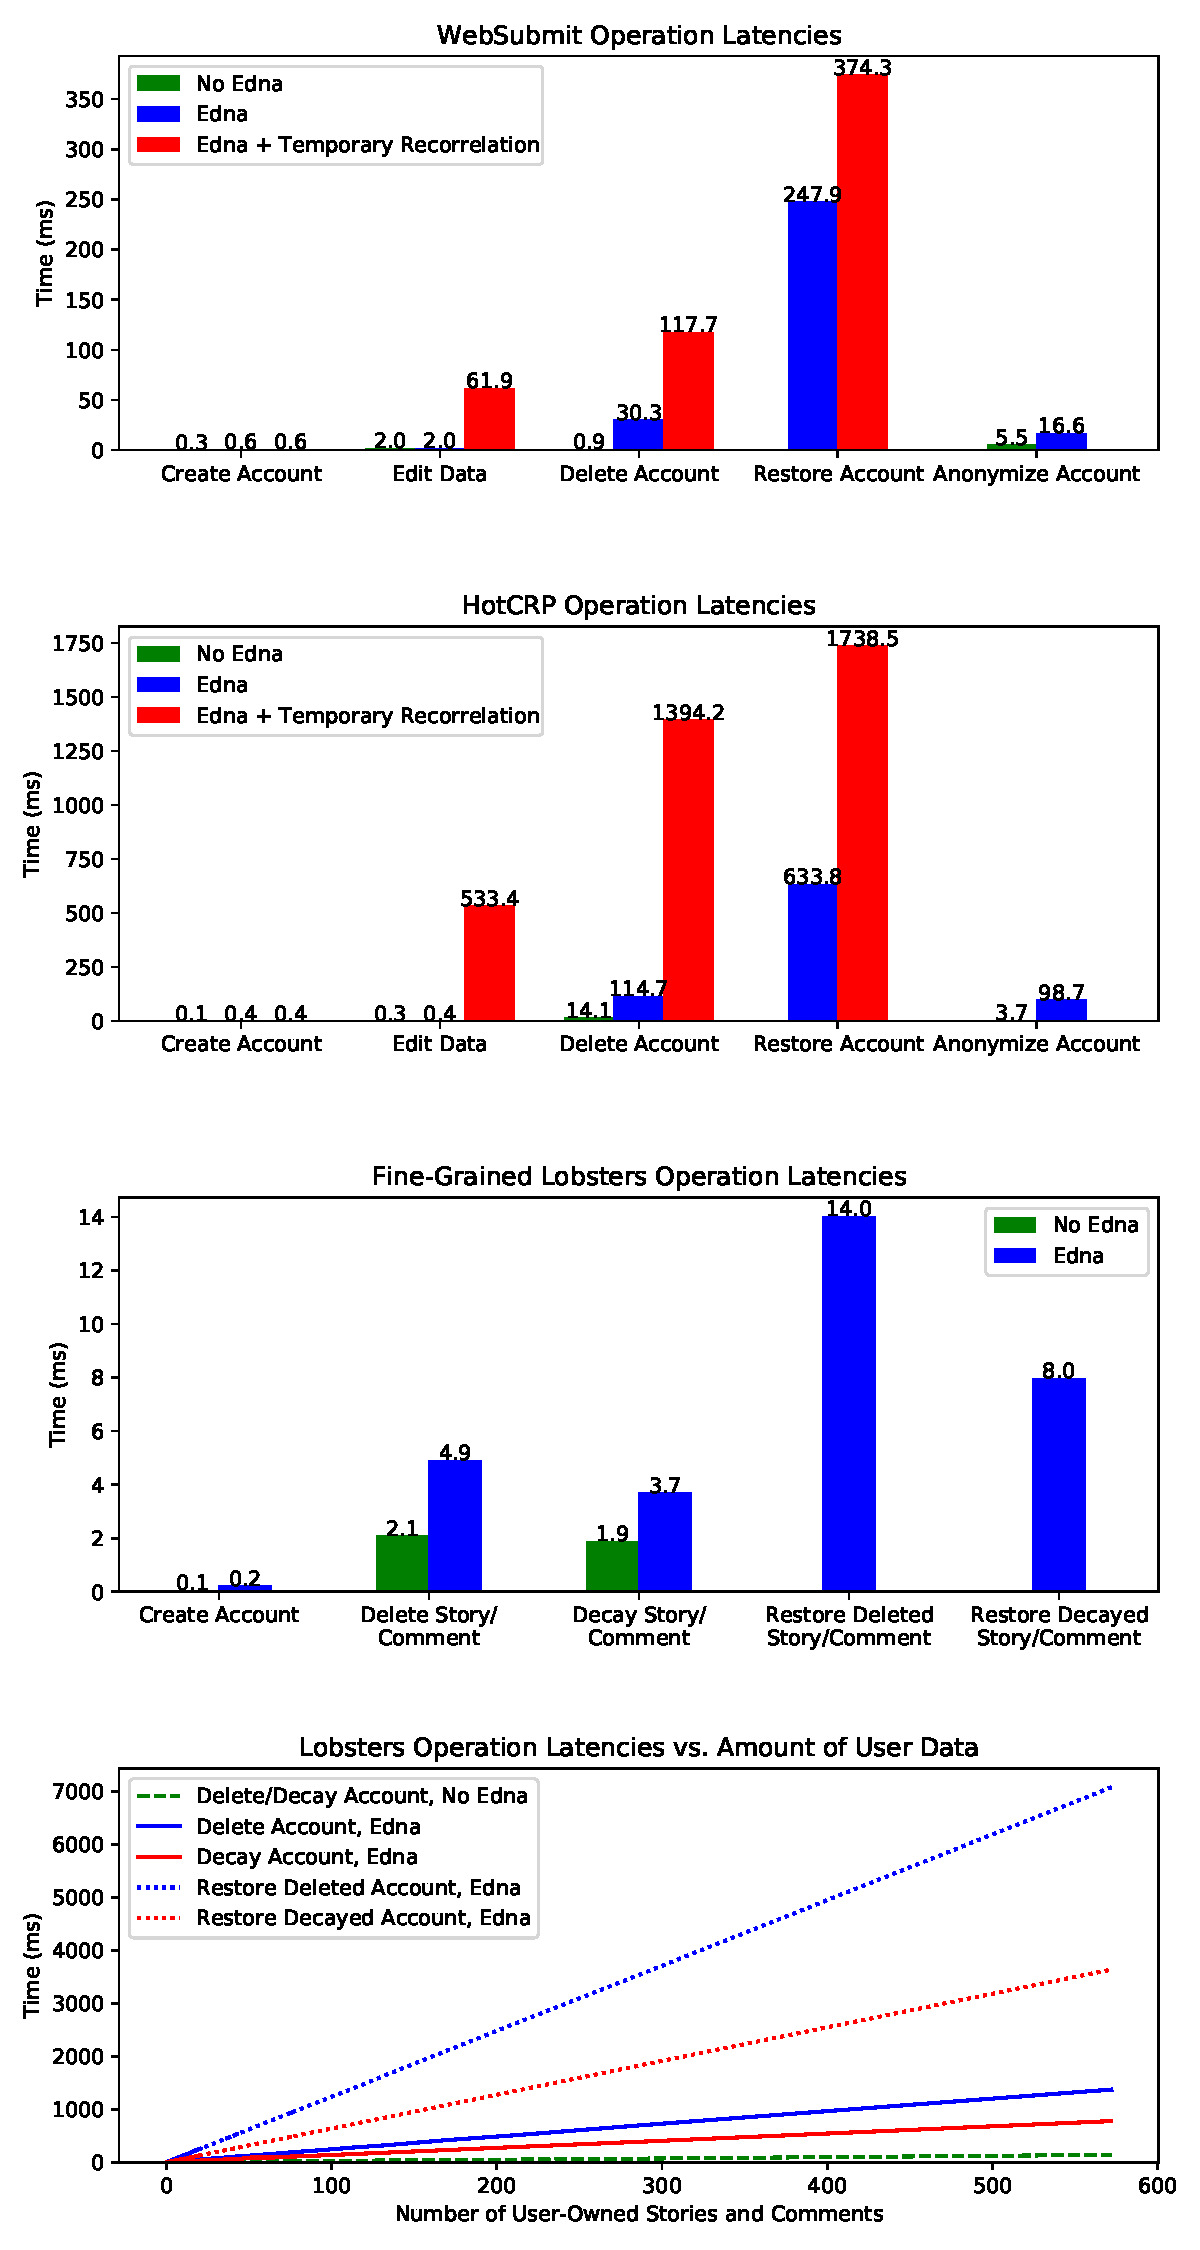
\includegraphics[width=0.5\textwidth]{figs/client_op_stats}
    \caption{Latencies of disguise-related actions when implemented manually by the
    application developer without \sys, and with \sys.
    Each bar shows the median latency; ranges indicate the 5th to 95th
    percentile latencies.}
    \label{fig:client_opstats}
\end{figure}

\begin{table*}[h!]
\begin{center}
\begin{tabular}{ c c }
\textbf{DB Op} & \textbf{Time (ms)}\\
\hline
Update DB Row & 0.1\\
Select DB Rows & 0.2\\
Remove DB Rows & 0.2\\
Reveal Deleted Row (DB Select + Insert) & 0.2 \\
Create + Register Principal & 0.1\\
\end{tabular}
\quad
\begin{tabular}{ c c }
\textbf{Crypto Op} & \textbf{Time (ms)}\\
\hline
Generate Keypair & 301\\
Encrypt SpeaksFor Record & 0.4\\
Decrypt SpeaksFor Record & 3.0\\
Encrypt Diff Record & 0.3\\
Decrypt Diff Record & 3.0\\
\end{tabular}
\end{center}
\caption{Amount of time required to run different operations required to apply and reveal disguises.}
\label{tab:opstats}
\end{table*}

\paragraph{WebSubmit.}
%
We run WebSubmit benchmarks with a database seeded with 2,000 users, 20
lectures with four questions each, and an answer for each question for
each user (160k total answers).
%
This might correspond to all classes in a department, or to a large AI class.
%
We measure end-to-end latency, which includes request processing in WebSubmit,
\sys's operations, and the response to the client.
%
The amount of data under disguise is constant across users, so we would expect
low variance in the results.
%

%
Figure~\ref{fig:websubmit-ops} shows the median latency for two normal operations
(creating an account and editing unanonymized data), two disguises (delete account
and anonymizing an account), and two operations over data under disguise (editing
anonymized data and restoring the account).
%
Normal operations have comparable latencies with and without \sys.
%

%
\sys's disguise-based account deletion takes 2.9ms, \vs 0.9ms in the manual
baseline.
%
This makes sense, as \sys encrypts database diffs and speaks-for records, while
the baseline only deletes data from the application DB.
%
The difference is greater for account anonymization, where \sys takes 10.8ms,
while the baseline takes less than 0.1ms.
\ms{why?}
%
Finally, \sys enables operations over data under disguise, which are impossible in
the baseline; these take 10.2ms and 21ms, well within acceptable interactive
latencies for web applications.
%
The simplicity of WebSubmit's disguises---which touch at maximum two database
tables---lead to fairly low latencies even for involved operations such as
restoring a deleted account (21ms).
%

\paragraph{HotCRP.}
%
We run the HotCRP experiments on a database seeded with 450 total users (50 of
whom are PC members), 450 papers, and four reviews and four comments per paper,
distributed evenly among PC members.
%
The benchmark measures the server-side latency to perform disguising and
application operations.
%
HotCRP supports the same disguise-related operations as WebSubmit.
%

HotCRP reviewers have slightly more variable amounts of data \lyt{TODO?} depending on the
assignment of papers to reviewers. HotCRP's disguises are far more complex than
WebSubmit's, touching 12 tables, and performing a mix of deletions and
decorrelations, leading to higher median latencies in general, even for the baseline.


\paragraph{Lobsters.}
%
We run Lobsters benchmarks on a database seeded with 14.5k users, which
is the late-2021 size of the real Lobsters site.
%
These users have \note{40k} stories, and \note{120k} comments with votes;
stories, comments, and votes are distributed among users according to
statistics from the actual Lobsters deployment~\cite{lobsters-data}.
%
The benchmark measures server-side latency of disguising and application
operations.
%

Lobsters supports account creation and deletion/restoration as well, but has account decay (and
subsequent restoration) instead of account anonymization.  It does not support editing anonymized
data (accounts can be restored in order to edit decorrelated data). In these benchmarks, we measure
the cost of GDPR-compliant account deletion and restoration.


Lobsters users' amount of data follows a skewed distribution, with most of the 5000 users
having fewer than 10 stories and comments, and a handful of users having over 300 stories and
comments. Lobster supports more complex disguises than WebSubmit and HotCRP,
touching 15 tables, and performing a mix of deletions, decorrelations, and modifications. This leads
to a higher latency as the amount of user data grows comparable to that of users in HotCRP and
WebSubmit.

\note{XXX old, unedited text follows. Malte is editing here.}

\paragraph{Drill-Down.}
%
Latency-critical tasks such as editing (unanonymized) data or
creating an account are largely unaffected by \sys.
%
To explain these costs, we break them down into fine-grained operations shown in
Table~\ref{tab:opstats}: every disguise action requires some DB operations and,
if using \sys, may require cryptographic operations.

\textbf{Creating an account} with or without \sys performs a database insert. Using \sys additionally
requires registering the new user as a principal, which assigns the user a (pre-generated)
private-public key pair, stores metadata about the new principal's key in \sys's storage, and
returns the corresponding private key to the application.
Using \sys thus incurs only the cost of an extra database operation, since the high cost of key
generation is taken offline.

\textbf{Editing data} with or without \sys simply performs database updates. Editing anonymized
data, however, requires \sys to decrypt (with the client-provided decryption capability) \emph{all}
speaks-for records at the client-provided locator until it finds a speaks-for record linking the
client to the currently-owning pseudoprincipal.  For example, if anonymization of a user account
generates 20 speaks-for record ciphertexts at the same locator, then editing anonymized data may
perform up to 20 decryptions to determine which pseudoprincipals the client can act for.

\textbf{Account deletion or data decay} with or without \sys performs the same database operations
to remove, modify, or anonymize data. \sys incurs increased costs by additionally encrypting and
inserting one diff record for each deleted or modified object, and one speaks-for record for each
anonymized object.

\textbf{Account restoration} is only possible with \sys. \sys decrypts a record for each
piece of modified/removed/anonymized data, and performs database checks to ensure the data can be restored
(\eg that the corresponding lecture of an answer to reinsert still exists). If the checks pass
(which they do in this benchmark), \sys restores the data stored in the diffs.

\textbf{Anonymization} with or without \sys generates one pseudoprincipal per object to anonymize
(\eg answers for lectures in WebSubmit, or reviews in HotCRP). Anonymization selects the relevant answers
to anonymize, generates new pseudoprincipals, and performs DB queries to insert new pseudoprincipals
and to update objects to point to these new pseudopricipals (\eg updating foreign keys).
\sys incurs increased costs by additionally generating per-pseudoprincipal speaks-for records, and
encrypting and storing these speaks-for records with the appropriate public keys.

\begin{figure}[t]
    \centering
    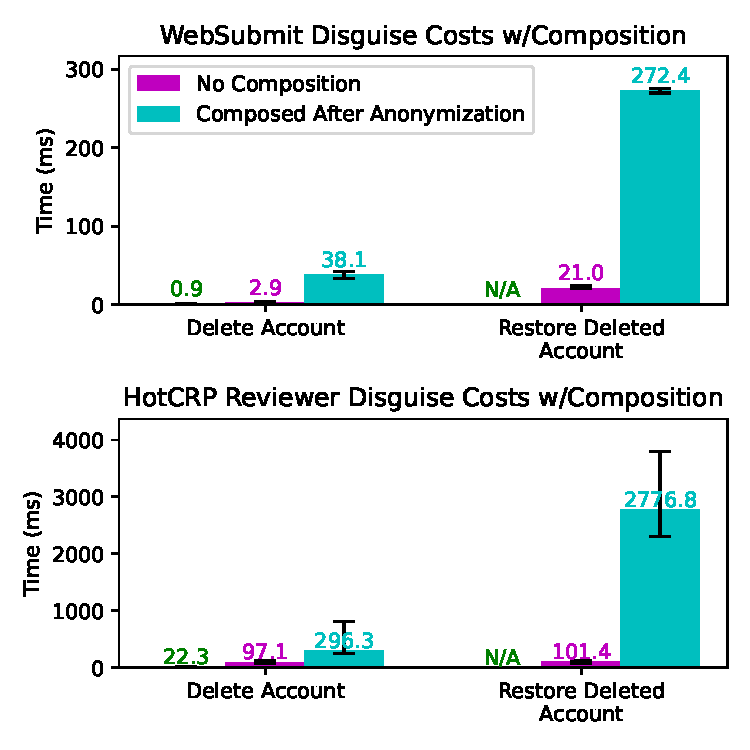
\includegraphics[width=0.45\textwidth]{figs/composition_stats}
    \caption{Latency of account delete and restore before anonymization vs. composed after anonymization.}
    \label{f:composition}
\end{figure}

\begin{figure*}[t]
    \centering
        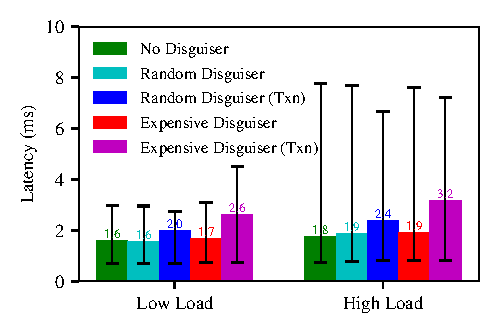
\includegraphics[width=0.45\textwidth]{figs/lobsters_concurrent_results}
        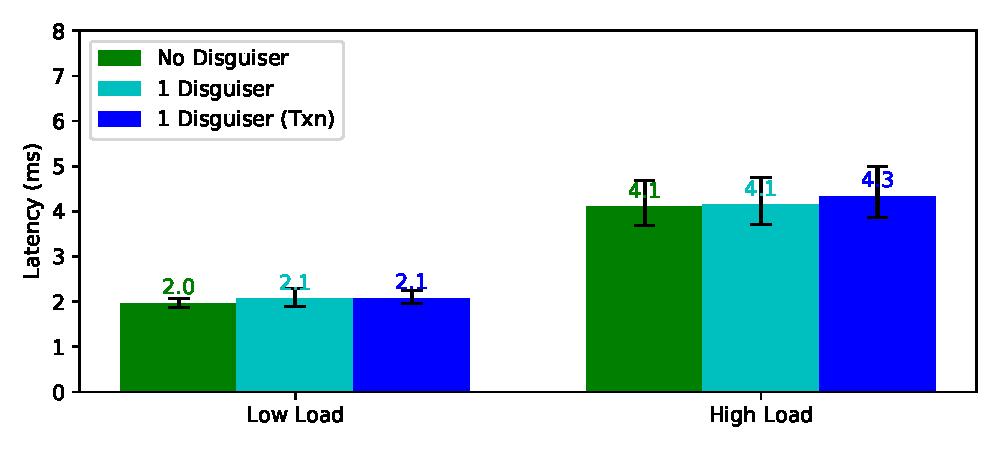
\includegraphics[width=0.45\textwidth]{figs/websubmit_concurrent_results}
    \caption{Impact of continuously applying and revealing account deletion disguises (non-transactional and transactional) on users concurrently running
    normal application operations. We show the median latency; ranges indicate the 5th to 95th
    percentile latencies.
    \textbf{Left (Lobsters)} tests the normal Lobsters traffic in the presence of an expensive
    disguiser (owning >6000 data objects) and a cheap disguiser (ownering <10 data objects). Even an expensive disguiser has minimal impact when user load is low; however, the impact increases as the server load increases, and if the
    disguise is transactional.
    \textbf{Right (WebSubmit)} tests an adversarial, write-only user workload of edits that
    modify the same table. All users have approximately the same amount of data (4 answers for 20
    lectures), and one user is chosen to continuously delete and restore their account. Here,
    disguising has minimal impact on latency even at high load.
    }
    \label{fig:concurrent}
\end{figure*}

\textbf{Composing Deletion After Anonymization.}
\lyt{TODO}
Account deletion post-anonymization requires \sys to perform temporary recorrelation find data of
pseudoprincipals that the user is authorized to remove along with their account. \sys incurs latency
increases from decrypting all speaks-for records of the user, and from performing the deletion or
modification queries for each discovered pseudoprincipal (in addition to the original user).

Account restoration may also restore pseudoprincipal-associated data, which requires temporary
recorrelation to access to pseudoprincipal-associated records produced from the account deletion.
\sys thus additionally decrypt speaks-for records for all pseudoprincipals of the user, which causes
the the increase in latency.\lyt{Numbers?}

%%%%%%%%%%%%%%%%%%%%%%%%%%%%%%%%%%%%%%%%%%%%%%%%%%%%%%%%%%%%%%%%%%%%%%%%
\subsection{Resource Use}
\label{s:eval-res}

Each generated pseudoprincipal adds an additional row to the users table in WebSubmit; \sys also
stores public-key metadata for each principal (and pseudoprincipal), and (in-memory) encrypted
ciphertexts for records.  Clients keep track of capabilities and locators that are emailed to them in
the form of URLs that allow for account restoration or post-anonymization editing.

%%%%%%%%%%%%%%%%%%%%%%%%%%%%%%%%%%%%%%%%%%%%%%%%%%%%%%%%%%%%%%%%%%%%%%%%
\subsection{Impact on Normal Application Use}
\label{s:eval-conc}

Figure~\ref{fig:concurrent} shows the impact of concurrently-running disguise actions on the latency
of normal application operations.

We first test the impact of disguising in Lobsters. We first achieve ~80\% CPU load by running
30 threads that model production Lobsters traffic. These threads simulate performing different
Lobsters operations (\eg loading the front-page, posting stories) according to measured access
frequencies and popularity distributions in production\lyt{CITE}. In this workload, 85\% of all
operations are front-page loads, which fetching stories and vote counts.

An additional number of threads simulate disguising users: these users (in the worst-case) decide to
simultaneously delete their account (\eg in response to some social media campaign). At some later
point in time, these users decide to come back and (in the worst case) simultaneously restore their
accounts.
We observe that even when the number of disguisers increases to 100, the latency of normal Lobsters
operation remains unaffected.

We then test an adversarial, write-only workload with WebSubmit. As a baseline, we achieve ~60\% CPU
load by running 100 threads that each continuously edit a user's lecture answers with 250-500ms
pauses between edits. This write-heavy workload achieves particularly high contention because all
edit queries modify the same database table; MySQL uses table-level locking for \texttt{MEMORY}
tables.

We then add an additional number of threads to simulate simultaneously disguising users.  While
fewer than 16 users disguising themselves at once has minimal impact on edit latency, 30 users doing
so causes spikes up to 4000ms.  These spikes come in pairs, with the larger second spike in the pair
coinciding with concurrent revealing (and the first of the pair coinciding with disguising);
revealing has greater impact due to its higher latency and compute costs.
%
Record batching improves these results by reducing the load generated by disguise actions: latency
spikes decrease to under 1500ms.

While we focus on normal application operation latency, we note that
disguise operation latency increases proportional to the overall system load (\eg due to MySQL’s
table-level locking). But this is acceptable, as disguises aren't time critical; in practice, they
still complete within a few seconds even at 60-80\% system load.
%
What matters is that normal application requests have acceptably low latency even in the presence of
disguising, which we achieve under realistic workloads (largely reads, with queries dispersed among
tables). If the workload becomes adversarial, \sys can prevent normal operation latency spikes by
rate-limiting disguise actions.

\section{Discussion}

\lyt{Should we note somewhere that pseudoprincipals and recursive disguising are why we need asymmetric
crypto; otherwise, we could just send the symmetric key to the original user being disguised?}

\lyt{
An alternative design might remove encrypted records completely (and \eg store them in external per-user
vaults or email them to the client).
This leaves no trace in \sys or the application, and would prevent the attacker from learning
anything. However, this places a large burden on the client.
Maybe put this in future work?
}

\ms{Hiding bag sizes -- very expensive, as would need to pad to max user data size, or add noise
proportional to that. Likely impractical.}


%-------------------------------------------------------------------------------
\printbibliography

%%%%%%%%%%%%%%%%%%%%%%%%%%%%%%%%%%%%%%%%%%%%%%%%%%%%%%%%%%%%%%%%%%%%%%%%%%%%%%%%
\end{document}
%%%%%%%%%%%%%%%%%%%%%%%%%%%%%%%%%%%%%%%%%%%%%%%%%%%%%%%%%%%%%%%%%%%%%%%%%%%%%%%%

%%  LocalWords:  endnotes includegraphics fread ptr nobj noindent
%%  LocalWords:  pdflatex acks
